%牛顿—莱布尼兹公式

\pentry{不定积分\upref{Int},定积分\upref{DefInt}}

牛顿—莱布尼兹公式描述了定积分和不定积分的关系.我们已知不定积分是求导的逆运算,而定积分是函数曲线下方的面积,二者乍看起来没什么联系,但牛顿—莱布尼兹公式却揭示了了二者之间的重要关系.

若 $F(x)$ 是 $f(x)$ 的一个原函数\upref{Int},则
\begin{equation}\label{NLeib_eq1}
\int_a^b f(x) \dd{x}  = F(b) - F(a)
\end{equation}

\subsection{推导}
\begin{figure}[ht]
\centering
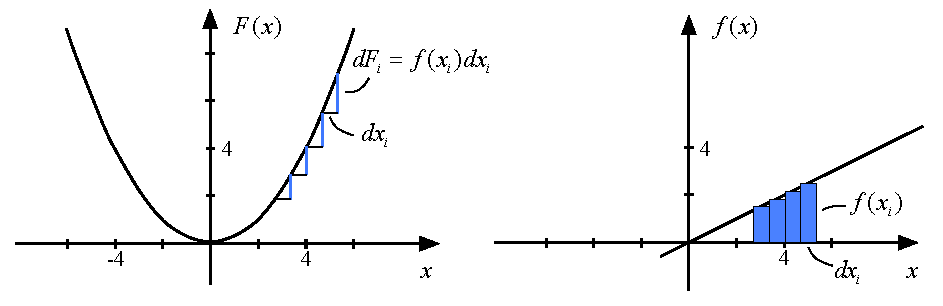
\includegraphics[width=13cm]{./figures/NLeib1.pdf}
\caption{右图中 $f(x)$ 的原函数为左图中的 $F(x)$, 当步长趋近0时,右图中的长方形面积趋近于左图中小竖线的长度.}\label{NLeib_fig1}
\end{figure}

如\autoref{NLeib_fig1}, 根据定积分\upref{DefInt} 的定义,有\footnote{这里假设极限存在.}
\begin{equation}
\int_a^b f(x) \dd{x}= \lim_{\Delta x_i\to 0}\sum_i f(x_i)\Delta x_i
\end{equation}
其中 $f(x_i)\Delta x_i$ 可看成是右图中第 $i$ 个小矩形的面积,求和是对从 $a$ 到 $b$ 的所有小矩形求和.现在不妨把 $x_i$ 设为第 $i$ 个小矩形左端的 $x$ 坐标. 考虑到求导是不定积分的逆运算,有 $f(x_i)=F'(x_i)$, 所以小矩形的面积变为
\begin{equation}
f(x_i)\Delta x_i = F'(x_i)\Delta x_i \approx \Delta F_i = F(x_{i+1})-F(x_i)
\end{equation}
最后一步使用了微分近似. %链接未完成
该式可以理解成,右图中的小矩形面积约等于左图中的小竖线长度,即原函数 $F(x)$ 在 $x_i$ 到 $x_{i+1}$ 间的增量.当取极限 $\Delta x_i \to 0$ 时,上式取等号.代回\autoref{NLeib_eq1}, 有
\begin{equation}
\int_a^b f(x) \dd{x}= \lim_{\Delta x_i\to 0}\sum_i [F(x_{i+1})-F(x_i)] = F(b)-F(a)
\end{equation}
该式可理解为,如果把左图中每一段 $\Delta x_i$ 所对应的微小增量 $\Delta F_i$ 都加起来,再取极限 $\Delta x_i \to 0$, 就是 $F(x)$ 从 $a$ 到 $b$ 的总增量. 在计算定积分的过程中, 为了书写简洁, 我们往往将上式中的 $F(b) - F(a)$ 记为 $\eval{F(x)}_a^b$.

\begin{exam}{计算定积分}
\begin{equation}
\int_{-l}^l \sin[2](\frac{n\pi}{l} x) \dd{x}
\end{equation}

\begin{figure}[ht]
\centering
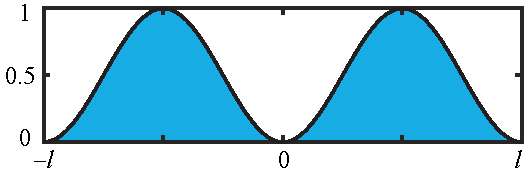
\includegraphics[width=8cm]{./figures/NLeib2.pdf}
\caption{$y = \sin[2](\pi x/l)$ 的定积分}\label{NLeib_fig2}
\end{figure}

先计算对应的不定积分.由积分表\upref{ITable} 中的\autoref{ITable_eq13} 结合\autoref{ITable_eq1} 得不定积分为
\begin{equation}
\int\sin^2(\frac{n\pi}{l} x) \dd{x} = \frac{l}{2n\pi} \qty[\frac{n\pi}{l} x - \sin(\frac{n\pi}{l} x)\cos(\frac{n\pi}{l} x)]
\end{equation}
再利用牛顿—莱布尼兹公式求定积分结果为 l. 计算该定积分还有另一种更简单的几何方法(见\autoref{NLeib_fig2}),由于被积函数的对称性,函数曲线可将区间 $[-l,l]$ 内高为 1 的长方形(面积为 $2l$ )划分成等面积的上下两部分,曲线下方的面积 $l$ 就是定积分的结果.
\end{exam}

\begin{exam}{圆的面积}\label{NLeib_ex2}
现在我们可以用\autoref{DefInt_ex2}\upref{DefInt} 中列出的两个定积分计算圆的面积. 先看第一个定积分, 由积分表\autoref{ITable_eq14} 得
\begin{equation}
\int \sqrt{R^2 - x^2} \dd{x} = \frac12 \qty(x\sqrt{R^2 - x^2} + R^2\arcsin\frac{x}{R}) + C
\end{equation}
由牛顿—莱布尼兹公式, $-R$ 到 $R$ 的定积分为 $\pi R^2/2$, 所以圆的面积为 $\pi R^2$.

第二个定积分要简单得多, 由幂函数的积分\autoref{ITable_eq2} 和牛顿—莱布尼兹公式得
\begin{equation}
\int_0^R 2\pi r \dd{r} = \pi \eval{r^2}_0^R = \pi R^2
\end{equation}
\end{exam}